\documentclass[a4paper]{article}

\usepackage[utf8]{inputenc}
\usepackage{float}
\usepackage{graphicx}
\usepackage{subfig}

\begin{document}


\title{Lab 3: Rasterization}

\author{Karl Johan Andreasson \and Erik Fahlén}

\maketitle

\begin{figure}[H]
    \centering
    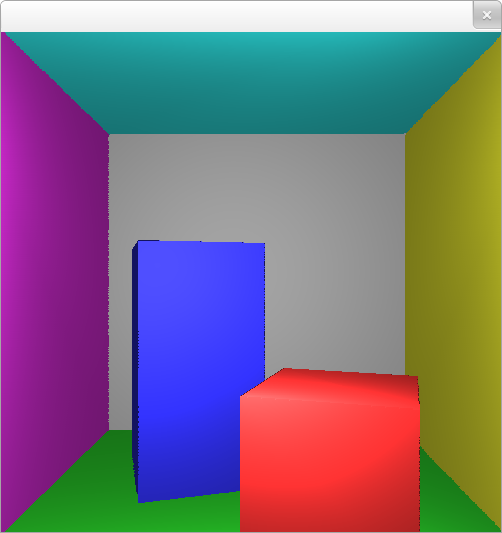
\includegraphics[width=6cm]{title.png}
    \caption{The scene rendered.}
    \label{fig:main}
\end{figure}

\section{Introduction}
As made evident in laboration 2 one has to be very clever about the
implementation when using raytracers to make it render in real time.

To combat these massive computation times required by the raytracer a common
implementation method in computer graphics is to use rasterization.
Rasterization will provide a much faster rendering time for each frame making
the scene being rendered in real time. The real time aspect of rasterization is
making it an ideal approach for applications such as computer games. It is in
fact the most used method to draw frames in computer games.

There are disadvantages of using a rasterization, such as that shadowing is much
harder to implement using rasterization than using ray tracing.

\section{Implementation method}

This laboration was implemented with both group members present and following
the instructions to implement the rasterizer.

Since many of the concepts were familiar to us from completing laboration one
and two the initial parts of the laboration was completed rather quickly. The
depth buffer provided some difficulties but these were figured out without too
much of a delay.

When the calculation of the index of the left most and right most pixels in a
row on the screen was calculated for a triangle there were some issues were 
these indices were out of bounds leading to us trying to read bad memory
positions. Once we implemented checks to disregard the parts of the triangles 
that were not on the screen these issues were fixed.

Even though we developed together, we still tracked the code with git.
This was useful when we wanted to return to an earlier version or if we
temporarily wanted to try two different things and see what worked best.

\section{Discussion}

This laboration was considerably more simple than laboration 2, mostly because they
were very similar. Some code could even be copied directly from the previous lab,
such as keyboard input and camera matrix code.

While projecting points and drawing lines in between them was something that we
already had the knowledge from the previous labs to do, the concept of filling
a polygon was new. The method used in this lab was not something that we
immedeatly would have thought of, but it is quite elegant once you realize how
it works. This was the main thing we learned in this lab, as shading and the other
components had mostly been covered by other labs or in the lectures.

One challange in this lab is that when calculatning the left and right pixel vectors,
you use pixel coordinates themselves as indices in the vectors. This means that if
you accidently do something wrong with your coordinates, you could start accessing
memory that you shouldn't and receive all sorts of strange errors. We managed to
overwrite our return adress from our method, making the application crash completely.
We ended up solving this by always doing range checks when accessing the vector.
This was a nice safe check that saved us from any difficult to find off-by-one errors.

Another slightly annoying thing about this lab is that the initial thing you do --
drawing edges between the vertices -- is not something that is left in the finished
product. This mostly felt like wasted time, since it was already things knew how to do
from the previous lab. It might be more necessary for someone who did not grasp the
3D space concepts perfectly before, since the next step of actually filling the
polygons is quite large.

One can question if the order of the last two laborations should be reversed. After
all, rasterization is more relevant to real-time graphics and should perhaps
be introduced earlier. Also, the results from the ray-tracer are more impressive,
so it might be more satisfying to do that last. They had about the same difficulty
level, so we don't think that the order matters very much from that perspective.


\section{Result}

At the given resolution of 500x500, our rasterizer runs at about 30 fps+. This
feels very responsive, making the real-time controls much more impressive than
in the ray-tracer.

As demonstrated in figure \ref{fig:camera} the camera can be moved around and
the view are as expected from a pin-hole camera.
Problems arise when objects are behind the camera. Distorted geometry might be
visible, or a few frames might take a really long time to render. This is due
to the fact that the polygons are projected wrongly and are really wide, making
the fill area much larger than the screen. While this never crashes the
application, it does take a long time to compute. All this is to be expected,
since clipping is not implemented.

The light source can be moved around as well, as specified in the lab instructions. A
demonstration of this can be seen in figure \ref{fig:light}. Note that geometry does
not block light. This is much more difficult to implement here than in the ray-tracer.

\begin{figure}[H]
    \centering
    \begin{minipage}{.5\textwidth}
        \centering
        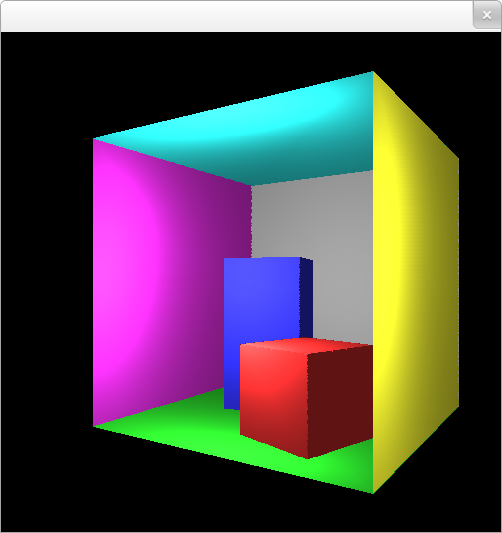
\includegraphics[width=4cm]{ani0.png}
    \end{minipage}%
    \begin{minipage}{.5\textwidth}
        \centering
        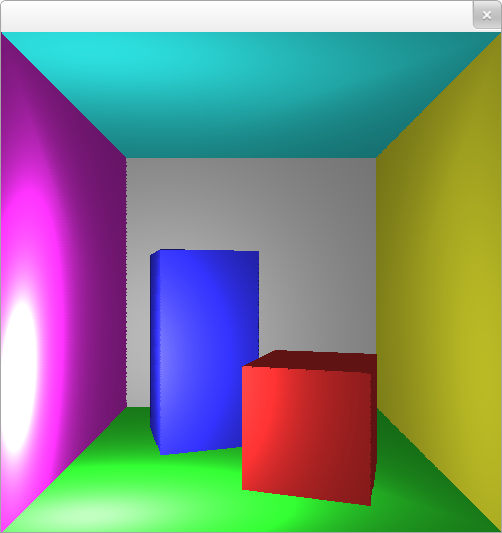
\includegraphics[width=4cm]{light0.png}
    \end{minipage}
\end{figure}

\begin{figure}[H]
    \centering
    \begin{minipage}{.5\textwidth}
        \centering
        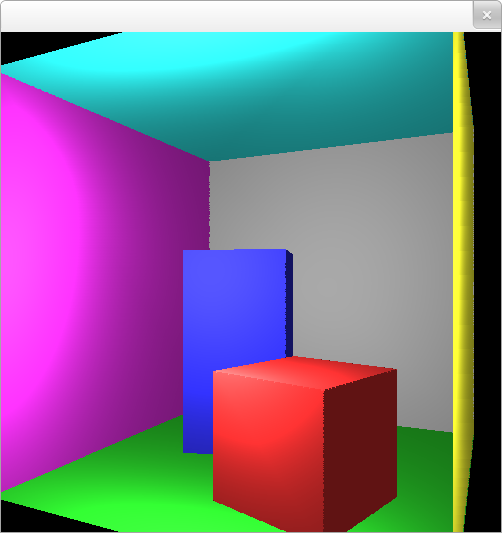
\includegraphics[width=4cm]{ani1.png}
    \end{minipage}%
    \begin{minipage}{.5\textwidth}
        \centering
        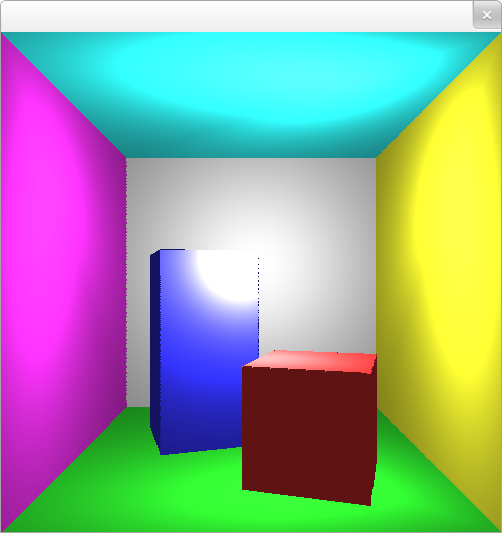
\includegraphics[width=4cm]{light1.png}
    \end{minipage}
\end{figure}

\begin{figure}[H]
    \centering
    \begin{minipage}{.5\textwidth}
        \centering
        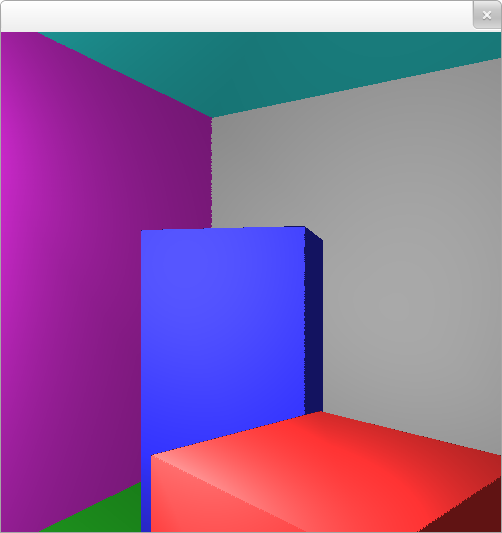
\includegraphics[width=4cm]{ani2.png}
        \captionof{figure}{\\Moving the camera around.}
        \label{fig:camera}
    \end{minipage}%
    \begin{minipage}{.5\textwidth}
        \centering
        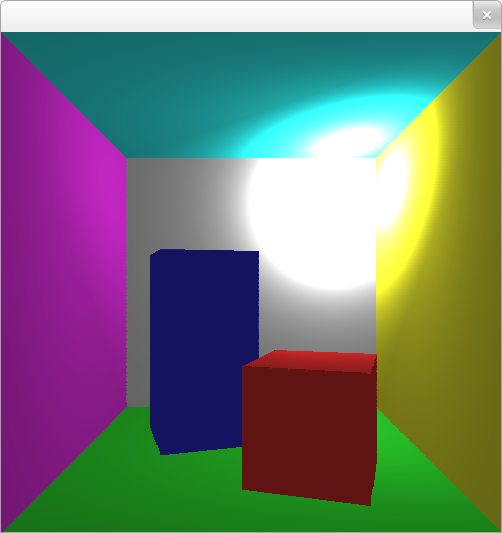
\includegraphics[width=4cm]{light2.png}
        \captionof{figure}{\\Moving the light source around.}
        \label{fig:light}
    \end{minipage}
\end{figure}

\end{document}
